% !TeX spellcheck = en_US
%% 字体:方正静蕾简体
%%		 方正粗宋
\documentclass[a4paper,left=2.5cm,right=2.5cm]{article}

\usepackage[utf8]{inputenc}
\usepackage{fontspec}
\usepackage{cite}
\usepackage{xeCJK}
\usepackage{tikz}
\usepackage{pgfplots}
\usepackage{indentfirst}
\usepackage{titlesec}
\usepackage{longtable}
\usepackage{graphicx}
\usepackage{float}
\usepackage{rotating}
\usepackage{subfigure}
\usepackage{tabu}
\usepackage{amsmath}
\usepackage{setspace}
\usepackage{amsfonts}
\usepackage{appendix}
\usepackage{listings}
\usepackage{xcolor}
\usepackage{geometry}
\setcounter{secnumdepth}{4}
\titleformat*{\section}{\LARGE}
\renewcommand\refname{参考文献}
%\titleformat{\chapter}{\centering\bfseries\huge\wryh}{}{0.7em}{}{}
%\titleformat{\section}{\LARGE\bf}{\thesection}{1em}{}{}
\titleformat{\subsection}{\Large\bfseries}{\thesubsection}{1em}{}{}
\titleformat{\subsubsection}{\large\bfseries}{\thesubsubsection}{1em}{}{}
\renewcommand{\contentsname}{{\cjkfzcs \centerline{目{  } 录}}}
\setCJKfamilyfont{cjkhwxk}{华文行楷}
%\setCJKfamilyfont{cjkfzcs}{方正粗宋简体}
\newcommand*{\cjkfzcs}{\CJKfamily{cjkfzcs}}
\newcommand*{\cjkhwxk}{\CJKfamily{cjkhwxk}}
\newfontfamily\wryh{Microsoft YaHei}
%\newfontfamily\ygyfryg{叶根友福荣银钩}
\newfontfamily\hwzs{华文中宋}
\newfontfamily\hwst{华文宋体}
\newfontfamily\hwfs{华文仿宋}
%\newfontfamily\jljt{方正静蕾简体}
\newfontfamily\hwxk{华文行楷}
\newcommand{\verylarge}{\fontsize{60pt}{\baselineskip}\selectfont}  
\newcommand{\chuhao}{\fontsize{44.9pt}{\baselineskip}\selectfont}  
\newcommand{\xiaochu}{\fontsize{38.5pt}{\baselineskip}\selectfont}  
\newcommand{\yihao}{\fontsize{27.8pt}{\baselineskip}\selectfont}  
\newcommand{\xiaoyi}{\fontsize{25.7pt}{\baselineskip}\selectfont}  
\newcommand{\erhao}{\fontsize{23.5pt}{\baselineskip}\selectfont}  
\newcommand{\xiaoerhao}{\fontsize{19.3pt}{\baselineskip}\selectfont} 
\newcommand{\sihao}{\fontsize{14pt}{\baselineskip}\selectfont}      % 字号设置  
\newcommand{\xiaosihao}{\fontsize{12pt}{\baselineskip}\selectfont}  % 字号设置  
\newcommand{\wuhao}{\fontsize{10.5pt}{\baselineskip}\selectfont}    % 字号设置  
\newcommand{\xiaowuhao}{\fontsize{9pt}{\baselineskip}\selectfont}   % 字号设置  
\newcommand{\liuhao}{\fontsize{7.875pt}{\baselineskip}\selectfont}  % 字号设置  
\newcommand{\qihao}{\fontsize{5.25pt}{\baselineskip}\selectfont}    % 字号设置 

\usepackage{diagbox}
\usepackage{multirow}
\usepackage{caption}
\boldmath
\XeTeXlinebreaklocale "zh"
\XeTeXlinebreakskip = 0pt plus 1pt minus 0.1pt
\definecolor{cred}{rgb}{0.8,0.8,0.8}
\definecolor{cgreen}{rgb}{0,0.3,0}
\definecolor{cpurple}{rgb}{0.5,0,0.35}
\definecolor{cdocblue}{rgb}{0,0,0.3}
\definecolor{cdark}{rgb}{0.95,1.0,1.0}
\lstset{
	language=matlab,
	numbers=left,
	numberstyle=\tiny\color{black},
	showspaces=false,
	showstringspaces=false,
	basicstyle={\footnotesize}\ttfamily,
	keywordstyle=\color{cdocblue}\bfseries,
	commentstyle=\color{cgreen},
	stringstyle=\color{cred},
	frame=lines,
	escapeinside=``,
	xleftmargin=1em,
	xrightmargin=1em, 
	%backgroundcolor=\color{cdark},
	aboveskip=1em,
	breaklines=true,
	tabsize=4
} 

\newfontfamily{\consolas}{Consolas}
\newfontfamily{\monaco}{Monaco}
\setmonofont[Mapping={}]{Consolas}	%英文引号之类的正常显示,相当于设置英文字体
\setsansfont{Consolas} %设置英文字体 Monaco, Consolas,  Fantasque Sans Mono
\setmainfont{Times New Roman}

\setCJKmainfont{华文中宋}

\newcommand*{\mytitle}
{
	
	\begingroup 
	\begin{center}
		\vspace*{0.05\paperheight} % White space at the top of the page
		\rule{\textwidth}{1.6pt}\vspace*{-\baselineskip}\vspace*{2pt} % Thick horizontal line
		\rule{\textwidth}{0.4pt}\\[\baselineskip] % Thin horizontal line
		{\yihao{\cjkhwxk {数学软件——短学期课程 \\[0.4\baselineskip]Matlab第二次作业}}}\\[0.2\baselineskip] % Title
		\rule{\textwidth}{0.4pt}\vspace*{-\baselineskip}\vspace{3.2pt}		
		\rule{\textwidth}{1.6pt}\\[3\baselineskip]
		
\includegraphics[width=0.5\textwidth]{xiaohui.jpg}
		\vspace*{3\baselineskip} % Whitespace between 
		{\LARGE\hwzs
			\begin{longtable}{ll}
				\cjkfzcs{姓名:}& 汪利军\\
				\cjkfzcs{学号:}& 3140105707\\
				\cjkfzcs{班级:}& 统计1401\\
			\end{longtable}
		}\par
		\vspace*{1\baselineskip}
		{\Large\hwzs 2016.07.11}
	\end{center}
	\vfill
	\endgroup
}
\usepackage{lastpage}
\usepackage{fancyhdr}
\pagestyle{fancy}
\lhead{\space \qquad \space}
\chead{数学软件——短学期课程 \qquad}
\rhead{\qquad\thepage/\pageref{LastPage}}
\begin{document}
	\begin{titlepage}
		\mytitle
	\end{titlepage}
	\begin{spacing}{1.5}
		
	\tableofcontents
	\end{spacing}
	\newpage
	\begin{spacing}{1.6}
		\section{问题重述}
		
		\begin{equation}
		\left\{
		\begin{array}{lll}
		-\nabla\cdot\Big(\dfrac{\nabla u}{|\nabla u|}\Big) & = & f\\
		u\Big|_{x=0} = 0,&& u\Big|_{y=0}=0\\
		\dfrac{\partial u}{\partial x}\Big|_{x=1}=y,&&\dfrac{\partial u}{\partial y}\Big|_{y=1}=x\\
		\Omega = [0,1]\times[0,1]
		\end{array}
		\right.
		\end{equation}
		
		已知精确解为
		\begin{equation}
		u(x,y)= xy
		\end{equation}
		
		于是
		\begin{eqnarray}
		f & = & - \nabla \cdot \Big(\dfrac{\nabla u}{|\nabla u|}\Big)\\
		& = & -\nabla \cdot \Big(\dfrac{y}{\sqrt{x^2+y^2}},\dfrac{x}{\sqrt{x^2+y^2}}\Big)\\
		& = & -\Big(-\frac{2xy}{(x^2+y^2)^{\frac{3}{2}}}\Big)\\
		& = & \frac{2xy}{(x^2+y^2)^{\frac{3}{2}}}
		\end{eqnarray}
		\section{有限差分推导}
		将$[0,1]$$N$等分,网格节点$0 = x_0<x_1<\cdots<x_N=1$
		\begin{center}
			\begin{tikzpicture}[scale = 1]
			\draw[gray, very thin] (0, 0) grid (12, 12);
			\foreach \x in {1, 2, 3}
			\draw[xshift = \x cm] node[below] {$\x$};
			\foreach \y in {1, 2, 3}
			\draw[yshift = \y cm] node[left] {$\y$};
			\foreach \x in {4, 4.2, ..., 10}
			\draw[xshift = \x cm] node[below] {$.$};
			\foreach \y in {4, 4.2, ..., 10}
			\draw[yshift = \y cm] node[left] {$.$};
			\foreach \x in {11}
			\draw[xshift = \x cm] node[below] {$N$};
			\foreach \x in {12}
			\draw[xshift = \x cm] node[below] {$N+1$};
			\foreach \y in {11}
			\draw[yshift = \y cm] node[left] {$N$};
			\foreach \y in {12}
			\draw[yshift = \y cm] node[left] {$N+1$};
			\end{tikzpicture}
			\captionsetup{font=footnotesize}
			\captionof{figure}{网格剖分}
		\end{center}
		\begin{equation}
		x_i = ih \qquad h = \frac{1}{N}
		\end{equation}
		\begin{eqnarray}
		(\frac{\partial u}{\partial x})_{ij} = \frac{u_{i+1,j}-u_{i-1,j}}{2h}+O(h^2)\\
		 (\frac{\partial u}{\partial y})_{ij} = \frac{u_{i,j+1}-u_{i,j-1}}{2h}+O(h^2)
		\end{eqnarray}
		\begin{eqnarray}
		&&\dfrac{\partial}{\partial x}\Big(\dfrac{1}{\big|\nabla u\big|}\frac{\partial u}{\partial x}\Big)_{ij} \\
		&=& \frac{1}{h}\Big[\frac{1}{\big|\nabla u\big|_{i+\frac{1}{2},j}}\big(\frac{u_{i+1,j}-u_{i,j}}{h}\big)-\frac{1}{\big|\nabla u\big|_{i-\frac{1}{2},j}}\big(\frac{u_{i,j}-u_{i-1,j}}{h}\big)\big] + O(h^2)\\
		&=&\dfrac{1}{h^2}\Big[\frac{1}{\big|\nabla u\big|_{i-\frac{1}{2},j}}u_{i-1,j}-(\frac{1}{\big|\nabla u\big|_{i-\frac{1}{2},j}}+\frac{1}{\big|\nabla u\big|_{i+\frac{1}{2},j}})u_{ij}+\frac{1}{\big|\nabla u\big|_{i+\frac{1}{2},j}}u_{i+1,j}\big]\\
		&&\frac{\partial}{\partial y}\Big(\frac{1}{\big|\nabla u\big|}\frac{\partial u}{\partial y}\big)_{ij} \\
		&=& \frac{1}{h}\Big[\frac{1}{\big|\nabla u\big|_{i,j+\frac{1}{2}}}\big(\frac{u_{i,j+1}-u_{i,j}}{h}\big)-\frac{1}{\big|\nabla u\big|_{i,j-\frac{1}{2}}}\big(\frac{u_{i,j}-u_{i,j-1}}{h}\big)\big] + O(h^2)\\
		&=&\dfrac{1}{h^2}\Big[\frac{1}{\big|\nabla u\big|_{i,j-\frac{1}{2}}}u_{i,j-1}-(\frac{1}{\big|\nabla u\big|_{i,j-\frac{1}{2}}}+\frac{1}{\big|\nabla u\big|_{i,j+\frac{1}{2}}})u_{ij}+\frac{1}{\big|\nabla u\big|_{i,j+\frac{1}{2}}}u_{i,j+1}\big]\\
		\end{eqnarray}
		则
		\begin{eqnarray}
		&&\nabla\cdot\Big(\frac{1}{\big|\nabla u\big|}\nabla u\Big)_{ij}\\
		&=&\dfrac{\partial}{\partial x}\Big(\dfrac{1}{\big|\nabla u\big|}\frac{\partial u}{\partial x}\Big)_{ij} + \frac{\partial}{\partial y}\Big(\frac{1}{\big|\nabla u\big|}\frac{\partial u}{\partial y}\big)_{ij} \\
		&=&\dfrac{1}{h^2}\Big[\frac{1}{\big|\nabla u\big|_{i-\frac{1}{2},j}}u_{i-1,j}+\frac{1}{\big|\nabla u\big|_{i+\frac{1}{2},j}}u_{i+1,j}+
		\frac{1}{\big|\nabla u\big|_{i,j-\frac{1}{2}}}u_{i,j-1}+
		\frac{1}{\big|\nabla u\big|_{i,j+\frac{1}{2}}}u_{i,j+1}\notag \\
		&&-
		(\frac{1}{\big|\nabla u\big|_{i-\frac{1}{2},j}}+\frac{1}{\big|\nabla u\big|_{i+\frac{1}{2},j}}+\frac{1}{\big|\nabla u\big|_{i,j-\frac{1}{2}}}+
		\frac{1}{\big|\nabla u\big|_{i,j+\frac{1}{2}}})u_{ij}
		\Big] + O(h^2)
		\end{eqnarray}
		
		\begin{eqnarray}
		\big|\nabla u\big|_{i-\frac{1}{2},j}
		&=&\Big|\Big(\big(\frac{\partial u}{\partial x}\big)_{i-\frac{1}{2},j},\big(\frac{\partial u}{\partial y}\big)_{i-\frac{1}{2},j}\Big)\Big|\\
		&=&\Big|\Big(\frac{u_{ij}-u_{i-1,j}}{h},\frac{u_{i-\frac{1}{2},j+1}-u_{i-\frac{1}{2},j-1}}{2h}\Big)\Big|
		\end{eqnarray}
		又
		\begin{equation}
		\left\{
		\begin{array}{lll}
		u_{i-\frac{1}{2},j\pm1} & =& u_{i-1,j\pm1}+\frac{1}{2}h\big(\frac{\partial u}{\partial x}\big)_{i-1,j\pm1}+O(h^2)\\
		& = & u_{i-1,j\pm1} + \frac{1}{2}h\cdot\frac{u_{i,j\pm1}-u_{i-2,j\pm1}}{2h} + O(h^2)\\
		& = & u_{i-1,j\pm1} + \frac{1}{4}(u_{i,j\pm1}-u_{i-2,j\pm1}) + O(h^2)\quad\text{当}i\neq 1\\
			u_{\frac{1}{2},j\pm1} &=& u_{1,j\pm1}-\frac{1}{2}h\cdot\frac{u_{2,j\pm1}-u_{0,j\pm1}}{2h}+O(h^2)\quad\text{当}i= 1\\
			&=&u_{1,j\pm1} - \frac{1}{4}u_{2,j\pm1}+O(h^2)\\
			u_{i-\frac{1}{2},0} &=& 0\qquad \text{当}j = 1
		\end{array}
		\right.
		\end{equation}
	%同理有
	%\begin{eqnarray}
	%u_{i-\frac{1}{2},j-1} & =& u_{i-1,j-1}+\frac{1}{2}h\big(\frac{\partial u}{\partial x}\big)_{i-1,j-1}+O(h^2)\\
	%& = & u_{i-1,j-1} + \frac{1}{2}h\cdot\frac{u_{i,j-1}-u_{i-2,j-1}}{2h} + O(h^2)\\
	%& = & u_{i-1,j-1} + \frac{1}{4}(u_{i,j-1}-u_{i-2,j-1}) + O(h^2)
	%\end{eqnarray}
	
	同理可求得
	%\begin{equation}
	%\big|\nabla u\big|_{i+\frac{1}{2},j},\big|\nabla %u\big|_{i,j-\frac{1}{2}},
	%\big|\nabla u\big|_{i,j+\frac{1}{2}}
	%\end{equation}
	\begin{eqnarray}
	\big|\nabla u\big|_{i+\frac{1}{2},j}
	&=&\Big|\Big(\big(\frac{\partial u}{\partial x}\big)_{i+\frac{1}{2},j},\big(\frac{\partial u}{\partial y}\big)_{i+\frac{1}{2},j}\Big)\Big|\\
	&=&\Big|\Big(\frac{u_{i+1,j}-u_{i,j}}{h},\frac{u_{i+\frac{1}{2},j+1}-u_{i+\frac{1}{2},j-1}}{2h}\Big)\Big|\\
	\big|\nabla u\big|_{i,j-\frac{1}{2}}
	&=&\Big|\Big(\big(\frac{\partial u}{\partial x}\big)_{i,j-\frac{1}{2}},\big(\frac{\partial u}{\partial y}\big)_{i,j-\frac{1}{2}}\Big)\Big|\\
	&=&\Big|\Big(\frac{u_{i+1,j-\frac{1}{2}}-u_{i-1,j-\frac{1}{2}}}{2h},\frac{u_{i,j}-u_{i,j-1}}{h}\Big)\Big|\\
	\big|\nabla u\big|_{i,j+\frac{1}{2}}
	&=&\Big|\Big(\big(\frac{\partial u}{\partial x}\big)_{i,j+\frac{1}{2}},\big(\frac{\partial u}{\partial y}\big)_{i,j+\frac{1}{2}}\Big)\Big|\\
	&=&\Big|\Big(\frac{u_{i+1,j+\frac{1}{2}}-u_{i-1,j+\frac{1}{2}}}{2h},\frac{u_{i,j+1}-u_{i,j}}{h}\Big)\Big|
	\end{eqnarray}

	以及
	\begin{equation}
	\left\{
	\begin{array}{lll}
	
	u_{i+\frac{1}{2},j\pm1} & =& u_{i,j\pm1}+\frac{1}{2}h\big(\frac{\partial u}{\partial x}\big)_{i,j\pm1}+O(h^2)\\
	& = & u_{i,j\pm1} + \frac{1}{2}h\cdot\frac{u_{i+1,j\pm1}-u_{i-1,j\pm1}}{2h} + O(h^2)\notag\\
	& = & u_{i,j\pm1} + \frac{1}{4}(u_{i+1,j\pm1}-u_{i-1,j\pm1}) + O(h^2)\notag\\
	u_{i\pm1,0} &=& 0	\quad\text{当}j=1\\
	u_{N+\frac{1}{2},j\pm1}&=&u_{N,n\pm1} + \frac{1}{2}hy_{i+1}
	\end{array}
	\right.
	\end{equation}
	
	类似地,
	\begin{equation}
	\left\{
	\begin{array}{lll}
	
	%u_{i+\frac{1}{2},j\pm1} & =& u_{i,j\pm1}+\frac{1}{2}h\big(\frac{\partial u}{\partial x}\big)_{i,j+1}+O(h^2)\\
	%& = & u_{i,j\pm1} + \frac{1}{2}h\cdot\frac{u_{i+1,j\pm1}-u_{i-1,j\pm1}}{2h} + O(h^2)\\
	%& = & u_{i,j\pm1} + \frac{1}{4}(u_{i+1,j\pm1}-u_{i-1,j\pm1}) + O(h^2)\\
	u_{i\pm1,j-\frac{1}{2}} & =& u_{i\pm1,j}-\frac{1}{2}h\big(\frac{\partial u}{\partial x}\big)_{i\pm1,j}+O(h^2)\\
	& = & u_{i\pm1,j} - \frac{1}{2}h\cdot\frac{u_{i\pm1,j+1}-u_{i\pm1,j-1}}{2h} + O(h^2)\notag\\
	& = & u_{i\pm1,j} - \frac{1}{4}(u_{i\pm1,j+1}-u_{i\pm1,j-1}) + O(h^2)\notag \\
	u_{0,j-\frac{1}{2}} &=& 0\quad\text{当}i=1\\
	u_{i\pm1,\frac{1}{2}} &=& u_{i\pm1,1}-\frac{1}{2}h\cdot\frac{u_{i\pm1,2}-u_{i\pm1,0}}{2h}+O(h^2)\\
	&=&u_{i\pm1,1} - \frac{1}{4}u_{i\pm1,2}+O(h^2)\quad\text{当}j = 1
	\end{array}
	\right.
	\end{equation}
	
	\begin{equation}
	\left\{
	\begin{array}{lll}
	u_{i\pm1,j+\frac{1}{2}} & =& u_{i\pm1,j}+\frac{1}{2}h\big(\frac{\partial u}{\partial x}\big)_{i\pm1,j}+O(h^2)\\
	& = & u_{i\pm1,j} + \frac{1}{2}h\cdot\frac{u_{i\pm1,j+1}-u_{i\pm1,j-1}}{2h} + O(h^2)\notag\\
	& = & u_{i\pm1,j} + \frac{1}{4}(u_{i\pm1,j+1}-u_{i\pm1,j-1}) + O(h^2)\notag \\
	u_{0,j+\frac{1}{2}} &=& 0\\
	%u_{i\pm1,N+\frac{1}{2}}&=&u_{i\pm 1,N}+
	\end{array}
	\right.
	\end{equation}
		为了表述方便.
		记
		\begin{eqnarray}
		p_1 = \frac{1}{h\big|\nabla u\big|_{i-\frac{1}{2},j}}\\
		p_2 = \frac{1}{h\big|\nabla u\big|_{i+\frac{1}{2},j}}\\
		p_3 = \frac{1}{h\big|\nabla u\big|_{i,j-\frac{1}{2}}}\\
		p_4 = \frac{1}{h\big|\nabla u\big|_{i,j+\frac{1}{2}}}
		\end{eqnarray}
		则有
		\begin{eqnarray}
		-\frac{1}{h^2}[p_1hu_{i-1,j}+p_2hu_{i+1,j}+p_3hu_{i,j-1}+p_4hu_{j,j+1}-(p_1+p_2+p_3+p_4)hu_{ij}]=f
		\end{eqnarray}
		从而有
		\begin{equation}
		(p_1+p_2+p_3+p_4)u_ij -p_1u_{i-1,j}-p_2u_{i+1,j}-p_3u_{j,j-1}-p_4u_{j,j+1} = hf
		\end{equation}
		
	\section{边界条件}
	
	\subsection{左边界}
	$i=1, 2\le j\le N-1$时,有
	\begin{equation}
	u_{i-1,j} = 0
	\end{equation}
	于是
	\begin{eqnarray}
	(p_1+p_2+p_3+p_4)u_{1j} - p_2u_{2j} - p_3u_{1,j-1} -p_4u_{1,j+1} &=& hf_{i,j} + p_1u_{0j} \\
	&=& hf_{i,j}
	\end{eqnarray}
	\subsection{右边界}
	$i=N,2\le j \le N-1$时,有
	\begin{equation}
	\frac{\partial u}{\partial x}\big|_{i+1,j} = y_{j}
	\end{equation}
	于是
	\begin{eqnarray}
	(p_1+p_2+p_3+p_4)u_{ij} - p_1u_{i-1,j} - p_3u_{i,j-1} - p_4u_{i,j+1} &=&hf_{i,j}+p_2u_{N+1,j}\label{right}\\
	&=& hf_{i,j} + {\color{red}p_2u_{N+1,j}}
	\end{eqnarray}
	对$u_{N,j}$进行泰勒展开
	\begin{eqnarray}
	u_{N,j} &=& u_{N+1,j} - \frac{1}{h}\frac{\partial u}{\partial x} + O(h^2) \\
	&=&u_{N+1,j} - \frac{1}{h}y_j
	\end{eqnarray}
	于是
	\begin{equation}
	u_{N+1,j} = u_{N,j} + \frac{1}{h}y_j \label{taylorright}
	\end{equation}
	从而,式(\ref{right})为
	\begin{eqnarray}
	&&(p_1+p_2+p_3+p_4)u_{ij} - p_1u_{i-1,j} - p_3u_{i,j-1} - p_4u_{i,j+1}\\ &=&hf_{i,j}+p_2u_{N+1,j}\\
	&=&hf_{i,j}+p_2(u_{N,j} + \frac{1}{h}y_j)
	\end{eqnarray}
	\subsection{上边界}
	$2\le i \le N-1,j=N$时,有
	\begin{equation}
	\frac{\partial u}{\partial x}\big|_{i,N+1} = x_i
	\end{equation}
	于是有
	\begin{eqnarray}
	&&(p_1+p_2+p_3+p_4)u_{iN} -p_1u_{i-1,N}-p_2u_{i+1,N}-p_3u_{i,N-1} \\
	&=&hf_{i,N}+{\color{red}p_4u_{i,N+1}}\label{up}
	\end{eqnarray}
	对$u_{i,N}$进行泰勒展开
	\begin{eqnarray}
	u_{i,N} &=& u_{i,N+1} - \frac{1}{h}\frac{\partial u}{\partial y} + O(h^2) \\
	&=&u_{i,N+1} - \frac{1}{h}x_{i}
	\end{eqnarray}
	于是
	\begin{equation}
	u_{i,N+1} = u_{i,N} + \frac{1}{h}x_{i} \label{taylorup}
	\end{equation}
	从而,式(\ref{up})为
	\begin{eqnarray}
	&&(p_1+p_2+p_3+p_4)u_{iN} - p_1u_{i-1,N} -p_2u_{i+1,N}- p_3u_{i+1,N}  \\ 
	&=&hf_{i,j}+p_4u_{i,N+1}\\
	&=&hf_{i,j}+p_4(u_{iN} + \frac{1}{h}x_{i})
	\end{eqnarray}
	\subsection{下边界}
	$2\le i \le N-1,j=1$时,有
	\begin{equation}
	u_{i,j-1}=0
	\end{equation}
	于是
	\begin{eqnarray}
	(p_1+p_2+p_3+p_4)u_{i1}-p_1u_{i-1,1}-p_2u_{i+1,j}-p_4u_{i,2}&=&hf_{i,j}+p_3u_{i,0}\\
	&=&hf_{i,j} 
	\end{eqnarray}
	\subsection{节点}
	\subsubsection{节点(1,1)}
	$i=1,j=1$时有
	\begin{eqnarray}
	u_{i-1,j} = 0\\
	u_{i,j-1} = 0
	\end{eqnarray}
	于是
	\begin{eqnarray}
	(p_1+p_2+p_3+p_4)u_{11} - p_2u_{21} - p_4u_{12} &=&hf_{x_1,y_1} + p_1u_{01} + p_3u_{10}\\
	&=&hf_{1,1}
	\end{eqnarray}
	\subsubsection{节点(1,N)}
	$i=1,j=N$时,有
	\begin{eqnarray}
	u_{i-1,j} = 0\\
	\frac{\partial u}{\partial y}\big|_{i,j+1} = x_{i}
	\end{eqnarray}
	于是
	\begin{eqnarray}
	(p_1+p_2+p_3+p_4)u_{1N}-p_2u_{2N} - p_3u_{1,N-1} &=&hf_{i,j}+p_1u_{0N} + p_4u_{1,N+1}\label{node_1n}\\
	&=&hf_{i,j}u_{0N}+{\color{red}p_4u_{1,N+1}}
	\end{eqnarray}
	对$u_{1,N}$进行泰勒展开有
	\begin{eqnarray}
	u_{1,N} &=& u_{1,N+1} - \frac{1}{h}\frac{\partial u}{\partial y} + O(h^2) \\
	&=&u_{1,N+1} - \frac{1}{h}x_1
	\end{eqnarray}
	于是
	\begin{equation}
	u_{1,N+1} = u_{1,N} + \frac{1}{h}x_1
	\end{equation}
	于是式(\ref{node_1n})为
	\begin{eqnarray}
	(p_1+p_2+p_3+p_4)u_{1N}-p_2u_{2N} - p_3u_{1,N-1} &=&hf_{i,j}+ p_4u_{1,N+1}\\
	&=&hf_{i,j}+p_4(u_{1,N}+\frac{x_1}{h})
	\end{eqnarray}
	\subsubsection{节点(N,1)}
	$i=N,j=1$时,有
	\begin{eqnarray}
	u_{N,j-1} = 0\\
	\frac{\partial u}{\partial x} \big|_{i+1,j} = y_j
	\end{eqnarray}
	于是有
	\begin{eqnarray}
	(p_1+p_2+p_3+p_4)u_{N1}-p_1u_{N-1,1} - p_4u_{N2} &=&hf_{i,j}+p_2u_{N+1,1} + p_3u_{N,0}\label{node_n1}\\
	&=&hf_{i,j}+{\color{red}p_2u_{N+1,1}}
	\end{eqnarray}
	对$u_{N1}$进行泰勒展开有
	\begin{eqnarray}
	u_{N1} &=& u_{N+1,1} - \frac{1}{h}\frac{\partial u}{\partial x} + O(h^2) \\
	&=&u_{N+1,1} - \frac{1}{h}y_1
	\end{eqnarray}
	于是
	\begin{equation}
	u_{N+1,1} = u_{N,1} + \frac{1}{h}y_1
	\end{equation}
	于是式(\ref{node_n1})为
	\begin{eqnarray}
	&&(p_1+p_2+p_3+p_4)u_{N1}-p_1u_{N-1,1} - p_4u_{N2}\\ &=&hf_{i,j}+p_2u_{N+1,1} \\
	&=&hf_{i,j}+p_2(u_{N,1}+\frac{y_1}{h})
	\end{eqnarray}
	\subsubsection{节点(N,N)}
	$i=N,j=N$时,有
	\begin{eqnarray}
	\frac{\partial u}{\partial x} \big|_{i+1,j} = y_j\\
	\frac{\partial u}{\partial y} \big|_{i,j+1} = x_i
	\end{eqnarray}
	于是
	\begin{eqnarray}
	&&(p_1+p_2+p_3+p_4)u_{NN} - p_1u_{N-1,N} - p_3u_{N,N-1}\label{nn}\\ &=&hf_{i,j}+p_2u_{N+1,N} + p_4u_{N,N+1}
	\end{eqnarray}
	由式(\ref{taylorright})及式(\ref{taylorup}),有
	\begin{eqnarray}
	u_{N+1,N} = u_{N,N} + \frac{1}{h}y_N\\
	u_{N,N+1} = u_{N,N} + \frac{1}{h}x_N
	\end{eqnarray}
	于是式(\ref{nn})可写成
	\begin{eqnarray}
	&&(p_1+p_2+p_3+p_4)u_{NN} - p_1u_{N-1,N} - p_3u_{N,N-1}\label{nn}\\
	&=&hf_{ij} +p_2(u_{NN}+\frac{1}{h}y_N)+p_4(u_{NN}+\frac{1}{h}x_N)
	\end{eqnarray}
	\section{系数矩阵}
	设$U=(u_{11},u_{21},\cdots,u_{N1},u_{12},\cdots,u_{N2},u_{13},\cdots,u_{N-1,N},u_{NN})'$,$A$为$N^2*N^2$的五对角矩阵.
	\begin{equation}
	A = 
	\left[
	\begin{array}{ccccccc}
		\sum\limits_{i=1}^{4}p_i&-p_2&\cdots&-p_4&\cdot&\cdots&\cdots\\
		-p_1&\sum\limits_{i=1}^{4}p_i&-p_2&\cdots&-p_4&\cdots&\cdots\\
		\vdots&-p_1&\sum\limits_{i=1}^{4}p_i&\cdots&\cdots&\cdots&\vdots\\
		\vdots&\vdots&\vdots&\vdots&\vdots&\vdots&\vdots\\
		-p_3& \cdots&\cdots&\cdots&\cdots&\cdots&\cdots\\
		\cdot& -p_3&\cdots&\cdots&\cdots&\cdots&\cdots\\
		\vdots&\vdots&\vdots&\vdots&\vdots&\vdots&\vdots\\
		\cdots&\cdots&\cdots&\cdots&\cdots&\cdots&\sum\limits_{i=1}^{4}p_i\\
	\end{array}
	\right]
	\end{equation}	
	根据上述边界条件的讨论,我们有
	\begin{equation}
	F_{ij}=\left\{
	\begin{array}{ll}
	hf_{ij} + p_2(u_{Nj}+\frac{1}{h}y_j) & i=N,2\le j \le N-1\\
	hf_{ij} + p_4(u_{iN}+\frac{1}{h}x_i) & j=N,2\le i \le N-1\\
	hf_{ij} + p_2(u_{NN}+\frac{1}{h}y_N)+p_4(u_{NN}+\frac{1}{h}x_N)& i=j=N\\
	hf_{ij}& others
	\end{array}
	\right.
	\end{equation}
	于是,我们的目标是求解线性方程
	\begin{equation}
	AU = F
	\end{equation}
	其中,
	$F=(F_{11},F_{21},\cdots,F_{N1},F_{12},\cdots,F_{N2},F_{13},\cdots,F_{N-1,N},F_{NN})'$。
	$A$中的$p_i$是根据上一步的值确定出来的,每次算出的$u$又作为下一步$p_i$的输入
	\end{spacing}
	\section{算法分析}
	由上述推导我们得出目标即是要求解方程$AU=F$,但$A$中含有与$u$有关的参数,于是想到先给$u$一个初值,不断迭代直至收敛到解。所以代码思路基本上是这样
	\begin{lstlisting}
	`给定初值u0`;
	`根据u0组装出系数矩阵A及F`;
	for lp = 1:maxIters
		u = A\F;
		err = norm(u-exu);
		if err < errStop
			break;
		end
		u0 = u;
	end
	plot;	
	\end{lstlisting}
	\section{运行结果}
	失败原因:
	\begin{figure}[H]
		\begin{figure}[H]
			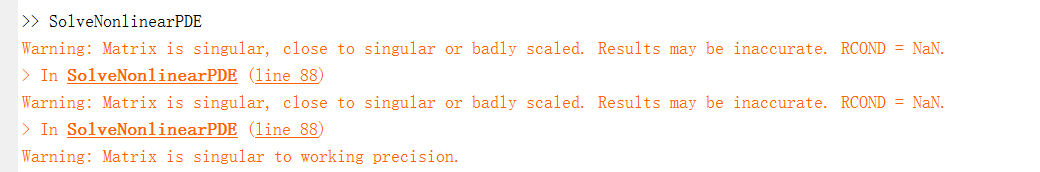
\includegraphics[width=\textwidth]{image/error.png}
			\caption{错误信息}
		\end{figure}
	\end{figure}
	时间有限,没有调试成功。
	\newpage
	\section*{附录}
	\begin{appendices}
		\textcolor[rgb]{0.98,0.00,0.00}{\textbf{代码如下:}}
		{\consolas\lstinputlisting{code/SolveNonlinearPDE.m}}
	\end{appendices}
\end{document}
